%%% Your header encountered errors when converting with LaTeXML
%%% Please uncomment it incrementally and check for problems
%%%   If you need assistance, contact us at help@authorea.com
%%% 
%
%\iflatexml
%% \documentclass[journal]{vgtc} % Not (yet) supported by LaTeXML.
%\fi
%                % final (journal style)
%% First macro on next line not (yet) supported by LaTeXML: 
%% \ifpdf%                                % if we use pdflatex
%  \pdfoutput=1\relax                     \pdfcompresslevel=9                    \pdfoptionpdfminorversion=7            \ExecuteOptions{pdftex}
%  \usepackage{graphicx}
%                % allow us to embed graphics files
%  \DeclareGraphicsExtensions{.pdf,.png,.jpg,.jpeg} \else  \ExecuteOptions{dvips}
%  \usepackage{graphicx}
%                % allow us to embed graphics files
%  \DeclareGraphicsExtensions{.eps}     \fi
%\graphicspath{{figures/}{pictures/}{images/}{./}}
%% \usepackage{microtype} % Not (yet) supported by LaTeXML.
%                 % use micro-typography (slightly more compact, better to read)
%\PassOptionsToPackage{warn}{textcomp}  % \usepackage{textcomp} % Not (yet) supported by LaTeXML.
%                  % use better special symbols
%\usepackage{mathptmx}
%                  % use matching math font
%% \usepackage{times} % Not (yet) supported by LaTeXML.
%                     % we use Times as the main font
%% First macro on next line not (yet) supported by LaTeXML: 
%% \renewcommand*\ttdefault{txtt}         % a nicer typewriter font
%\usepackage{cite}
%                      % needed to automatically sort the references
%% \usepackage{tabu} % Not (yet) supported by LaTeXML.
%                      % only used for the table example
%\usepackage{booktabs}
%                  % only used for the table example
%% First macro on next line not (yet) supported by LaTeXML: 
%% \onlineid{0}
%% First macro on next line not (yet) supported by LaTeXML: 
%% \vgtccategory{Research}
%% First macro on next line not (yet) supported by LaTeXML: 
%% \vgtcpapertype{please specify}
%% First macro on next line not (yet) supported by LaTeXML: 
%% \authorfooter{
%%%% insert punctuation at end of each item
%%\item
%% Roy G. Biv is with Starbucks Research. E-mail: roy.g.biv@aol.com.
%%\item
%% Ed Grimley is with Grimley Widgets, Inc.. E-mail: ed.grimley@aol.com.
%%\item
%% Martha Stewart is with Martha Stewart Enterprises at Microsoft
%% Research. E-mail: martha.stewart@marthastewart.com.
%%}
%% First macro on next line not (yet) supported by LaTeXML: 
%% \shortauthortitle{Biv \MakeLowercase{\textit{et al.}}: Global Illumination for Fun and Profit}
%% First macro on next line not (yet) supported by LaTeXML: 
%% \CCScatlist{ % not used in journal version
%% \CCScat{K.6.1}{Management of Computing and Information Systems}%
%%{Project and People Management}{Life Cycle};
%% \CCScat{K.7.m}{The Computing Profession}{Miscellaneous}{Ethics}
%%}
%% First macro on next line not (yet) supported by LaTeXML: 
%% \teaser{
%%  \centering
%%  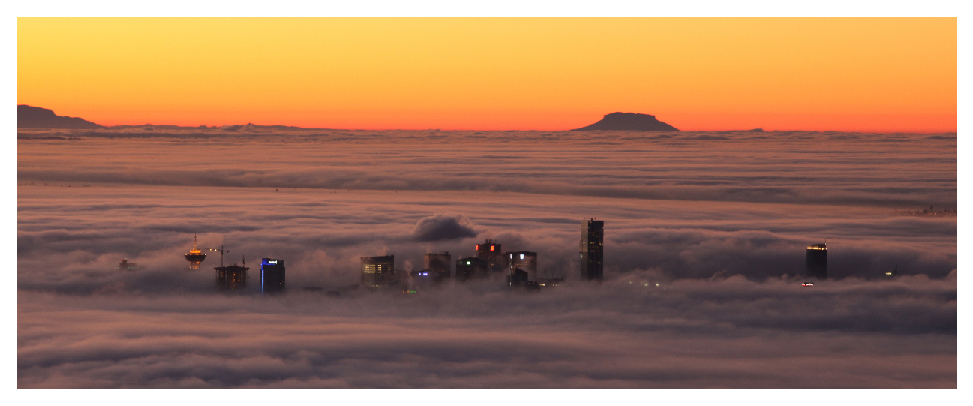
\includegraphics[width=\linewidth]{CypressView}
%%  \caption{In the Clouds: Vancouver from Cypress Mountain. Note that the teaser may not be wider than the abstract block.}
%%	\label{fig:teaser}
%%}
%% First macro on next line not (yet) supported by LaTeXML: 
%% \vgtcinsertpkg
